En el siguiente capítulo se desarollan las herramientas de gestión lean utilizadas en el proyecto además de exponer una breve explicación de la metodología y su implantación en los últimos años.

\section{Definición de la metodología lean}

La gestión Lean es un concepto moderno para la optimización de procesos en toda la cadena de valor \cite{helmold_progress_2019}.
Se centra en hacer que las ineficiencias, o desperdicios, sean transparentes y en alterarlas para convertirlas en actividades que añadan valor \cite{helmold_global_2016}.
La cadena de valor abarca en este contexto desde los proveedores, pasando por las propias operaciones, hasta los clientes \cite{slack_operations_2010}.
Las ineficiencias son todo aquello, por ejemplo, una actividad, un proceso y un producto, que se considera algo por lo que los clientes no están dispuestos a pagar o a gastar medios financieros.

El cliente es el punto central del concepto lean.
Los principales objetivos de la filosofía lean son crear valor para el cliente mediante la optimización de los recursos y crear un flujo de trabajo constante basado en las demandas reales de los clientes \cite{ohno_toyota_1988}. Busca eliminar cualquier pérdida de tiempo, esfuerzo o dinero identificando cada paso en un proceso de negocio y luego revisando o recortando los pasos que no crean valor \cite{bertagnolli_lean_2018}.

La filosofía tiene sus raíces en Japón y las operaciones, pero actualmente está ampliamente extendida por todo el mundo y las industrias.
Sus puntos centrales son los siguientes:

\begin{itemize}
    \item Poner al cliente en el centro de la operación.
    \item Definir el valor y el valor añadido desde el punto de vista del cliente final.
    \item Eliminar todos los residuos en todos los ámbitos de la cadena de valor.
    \item Mejorar continuamente todas las actividades, procesos, objetivos y personas.
    \item Situar a las personas en el centro de los servicios y procesos de valor añadido.
\end{itemize}

La gestión lean facilita el liderazgo y la responsabilidad compartida mientras que la mejora continua garantiza que cada empleado contribuya al proceso de mejora.
La metodología actúa como guía para construir una organización sólida y de éxito que progresa constantemente, identificando los problemas reales y resolviéndolos.
Lean se basa en el sistema de producción Toyota, creado a finales de los años cuarenta.
Toyota puso en práctica los cinco principios de la gestión ajustada con el objetivo de reducir la cantidad de procesos que no producían valor, lo que se conoce como \textit{Toyota Way}.

Al aplicar los cinco principios, se encontraton mejoras significativas en eficiencia, productividad, rentabilidad y duración de los ciclos.
Lean incorpora cinco principios rectores que son utilizados por los directivos de una organización como directrices de la metodología \cite{helmold_progress_2019}. Los cinco principios son:

\begin{itemize}
    \item Identificar el valor en todos los procesos de la cadena de valor.
    \item Realización de mapas de flujo de valor.
    \item Crear un flujo de trabajo continuo.
    \item Establecer un sistema \textit{pull} en el que los clientes sean el centro de atención.
\end{itemize}

Identificar el valor, el primer paso en la gestión lean, significa encontrar el problema que el cliente necesita resolver y convertir el producto en la solución.
En concreto, el producto debe ser la parte de la solución por la que el cliente esté dispuesto a pagar.
Cualquier proceso o actividad que no añada valor, es decir, que no aporte utilidad y el cliente no está dispuesto a pagar por ello, importancia o valor al producto fnal se considera residuo y debe eliminarse \cite{liker_toyota_2006}.

\textit{Value Stream Mapping} se refiere a la herramienta que se utiliza para mapear el flujo de trabajo de la empresa, incluyendo todas las acciones y personas que contribuyen al proceso de creación y entrega del producto final al consumidor.
Trazar la cadena de valor ayuda a los directivos a visualizar qué procesos están dirigidos por qué equipos y a identificar a las personas responsables de medir, evaluar y mejorar el proceso.
La visualización ayuda a los directivos a determinar qué partes del sistema no aportan valor al flujo de trabajo \cite{slack_operations_2010}.

Crear un flujo de trabajo continuo significa garantizar que el flujo de trabajo de cada equipo progrese sin problemas y evitar las interrupciones o cuellos de botella que pueden producirse con el trabajo en equipos interfuncionales.
\textit{Kanban}, una técnica de gestión ajustada que utiliza una señal visual para desencadenar la acción, se utiliza para facilitar la comunicación entre equipos para que puedan abordar lo que hay que hacer y cuándo hay que hacerlo.
En el proceso de trabajo total en una colección de partes más pequeñas y visualizar el flujo de trabajo en este sentido facilitan la eliminación factible de interrupciones y interrupciones y bloqueos.

Desarrollar un sistema \textit{pull} asegura que el flujo de trabajo continuo se mantenga estable y garantiza que los equipos entreguen las asignaciones de trabajo más rápido y con menos esfuerzo. Un sistema pull es una técnica lean específica que reduce los residuos de cualquier producción. Garantiza que sólo se inicie un nuevo trabajo si hay demanda del mismo, lo que ofrece la ventaja de minimizar los gastos generales y optimizar los costes de almacenamiento.

El último principio es la mejora continua y puede considerarse el paso más importante del método de gestión ajustada.
Facilitar la mejora continua se refiere a una serie de técnicas que se utilizan para identificar lo que una organización ha hecho, lo que necesita hacer, los posibles obstáculos que puedan surgir y cómo todos los miembros de la organización pueden mejorar sus procesos de trabajo.
El sistema lean no está aislado ni es inmutable, por lo que pueden surgir problemas en cualquiera de los otros cuatro pasos.
Asegurarse de que todos los empleados contribuyen a la mejora continua del flujo de trabajo protege a la organización cuando surgen problemas.
La dirección debe crear un entorno y una cultura en los que todos los empleados puedan trabajar de acuerdo con los cinco principios \cite{ohno_toyota_1988,bertagnolli_lean_2018}.

\section{La gestión lean en el sector sanitario}

Lean parte del rechazo al despilfarro. Atribuido a Taiichi Ohno, el sistema Lean se desarrolló en los años 50 y 60 para ofrecer la mejor calidad, el menor coste y el menor plazo de entrega mediante la eliminación de los residuos.
El término japonés para lo que las empresas estadounidenses suelen clasificar como despilfarro es \textit{muda} y fue definido por Fujio Cho de Toyota como "cualquier cosa que no sea la cantidad mínima de equipo, espacio y tiempo del trabajador, que son absolutamente esenciales para añadir valor al producto" \cite{helmold_lean_2020}.

La presencia de este tipo de residuos en un sistema repercute negativamente en el plazo de entrega, el coste y la calidad.
A principios de los años 80, empresas de otros sectores, como el sanitario, comprendieron que la introducción de los principios lean conllevaría varias ventajas.
El despilfarro en la sanidad puede describirse, entre otros elementos, en el transporte excesivo de medicamentos o pacientes, el tiempo de espera para los tratamientos o la infrautilización de equipos y máquinas en los hospitales. Además, las duplicaciones e ineficiencias del personal de enfermería también pueden repercutir en la creación de residuos.

Aunque la metodología de mejora empresarial lean se desarrolló inicialmente para mejorar la calidad y la productividad de las fábricas de automóviles, se ha utilizado con gran éxito en industrias y entornos de todo tipo, como el desarrollo de software, la administración pública, el comercio minorista y otros entornos de servicios.
Las organizaciones sanitarias, en particular, han descubierto que el enfoque puede utilizarse para reducir costes y mejorar la calidad y la satisfacción de los pacientes al mismo tiempo \cite{millard_how_nodate}.
Uno de los principios básicos del lean es la eliminación del despilfarro, que se define como todo aquello que no añade valor al cliente.
Los profesionales se centran en ocho tipos específicos de residuos.
Son tan comunes en la sanidad como en la industria.
Por lo tanto, la gestión ajustada tiene como objetivo eliminar, por ejemplo, los tiempos de espera o el exceso de medicación como se muestra en la Tabla~\ref{tab:timwood}.

\begin{table}
    \centering
    \begin{tabular}{llp{10cm}}
        \toprule
        Letra & Despilfarro     & Definición                                                                         \\
        \midrule
        T     & Transport       & Movimiento excesivo de personas, información o materiales                          \\
        I     & Inventory       & Stock excesivo y retraso en la información o productos                             \\
        M     & Motion          & Cualquier movimiento que no añada valor al producto o al proceso                   \\
        W     & Waiting         & Largos periodos de inactividad de personas, información, maquinaria o   materiales \\
        O     & Overutilization & Producir más o antes de que lo requiera el cliente                                 \\
        O     & Overmedication  & Utilización de las herramientas, procedimientos o sistemas incorrectos             \\
        D     & Defects         & Errores frecuentes en los trámites o en la calidad del producto                    \\
        \bottomrule
    \end{tabular}
    \caption{TIMWOOD, el acrónimo que define los siete despilfarros en el sector sanitario}
    \label{tab:timwood}
\end{table}

\subsection{Transporte}

El despilfarro del transporte se produce cuando los materiales se trasladan de un lugar a otro de forma ineficaz. En sanidad se produce cuando:

\begin{itemize}
    \item Los pacientes son trasladados de un departamento a otro o de una habitación a otra
    \item Los medicamentos se trasladan de la farmacia al lugar donde se necesitan
    \item Los suministros se trasladan del almacén a la planta
\end{itemize}

Algunos de estos transportes se consideran residuos "necesarios" que hay que minimizar aunque no puedan eliminarse por completo.

\subsection{Inventario}

Los fabricantes han adoptado en gran medida un enfoque de inventario justo a tiempo para reducir los costes relacionados con el almacenamiento, el movimiento, el deterioro y el desperdicio.
Las organizaciones sanitarias buscan hacer lo mismo en lo que se refiere a:

\begin{itemize}
    \item Medicación que esté cerca de la fecha de caducidad
    \item Exceso de consumibles
    \item Formularios preimpresos
    \item Exceso de material de cabecera
\end{itemize}

\subsection{Movimiento}

El movimiento se refiere al desplazamiento innecesario de personas dentro de una instalación.
Este ocurre cuando:

\begin{itemize}
    \item La distribución de las oficinas o del hospital no es coherente con el flujo de trabajo.
    \item Los suministros no se almacenan donde se necesitan
    \item Los equipos no están bien situados
\end{itemize}

El primer paso para combatir los despilfarros del lean es reconocerlos dentro de su organización.
En la mayoría de los casos, el examen de cada uno de estos factores específicos que contribuyen con frecuencia al despilfarro conduce al descubrimiento de múltiples oportunidades de mejora.
También podemos esforzarnos por eliminar el despilfarro (incluidos los clics del ordenador) en los sistemas de software.

\subsection{Esperas}

En la fabricación, la espera se produce cuando las piezas no pueden salir o cuando los miembros del equipo no pueden realizar sus tareas debido a problemas, como la falta de existencias o fallos en los equipos.
La espera en la atención sanitaria es un problema tanto para los pacientes como para los proveedores.

\begin{itemize}
    \item Pacientes en salas de espera (o de examen)
    \item Funcionarios con cargas de trabajo desiguales a la espera de su próxima tarea
    \item Pacientes de urgencias y médicos a la espera de los resultados de las pruebas
    \item Pacientes de urgencias en espera de ingreso hospitalario
    \item Pacientes en espera de alta médica
\end{itemize}

\subsection{Sobreutilización}

En la industria manufacturera, la sobreproducción se traduce en un exceso de ``trabajo en curso'' o de existencias de ``productos acabados'' sin vender.
En sanidad es más difícil de detectar, pero se produce cuando los proveedores hacen más de lo que necesita el cliente en ese momento.
Incluye:

\begin{itemize}
    \item Pruebas diagnósticas innecesarias
    \item Comidas no consumidas
    \item Pedir medicamentos que el paciente no necesita
    \item Personal en horas no punta
\end{itemize}

\subsection{Sobremedicación}

Sobreprocesar significa hacer más trabajo, hacerlo más complejo o más caro de lo necesario.
Adopta la forma de:

\begin{itemize}
    \item Pedir imágenes diagnósticas complejas (resonancia magnética) cuando bastaría con un método más sencillo (radiografía)
    \item Trámites innecesarios
    \item Intervención quirúrgica en lugar de una alternativa médica igualmente eficaz
    \item Citas de seguimiento que no mejoran los resultados del paciente
    \item Tratamientos por especialistas que podrían realizar los proveedores de atención primaria
\end{itemize}

\subsection{Defectos}

Mientras que los defectos de fabricación son caros y molestos, en la atención sanitaria pueden ser mortales.
Pueden incluir:

\begin{itemize}
    \item Diagnóstico erróneo
    \item Administración de medicamentos incorrectos
    \item Afecciones adquiridas en el hospital
    \item Códigos identificativos incorrectos
\end{itemize}

El despilfarro incluye el tiempo empleado en crear un defecto, reelaborar estos defectos e inspección de estos defectos.
Aunque consideremos que la inspección es un despilfarro, no podemos hasta que no tengamos un proceso perfecto sin defectos.
Incluso Toyota aún tiene inspecciones finales cada año, pero la consideran un despilfarro que esperan eliminar algún día.

\section{Estandarización de tareas}

El trabajo estandarizado es uno de los pilares de la metodología lean, sin embargo, su aplicación en entornos alejados de la industria manufacturera, como una oficina o un hospital puede ser no tan clara.
Las dificultades de su aplicación residen principalmente en el desconocimiento de los beneficios que puede aportar, sobre todo al no ser tangibles como podría ser si se estuviera fabricando un producto.
Entre los argumentos en contra del trabajo estandarizado se encuentran \cite{locher_lean_2017}:

\begin{itemize}
    \item ``¿Por qué preocuparse de cómo llevo a cabo mis tareas siempre y cuando se termine el trabajo?''
    \item ``El trabajo estandarizado no es efectivo para las actividades creativas en oficinas y servicios''
    \item ``El entorno de oficinas es demasiado variable y no es adecuado para estandarizar''
\end{itemize}

\subsection{Propósito de la estandarización}

La estandarización de las tareas es uno de los mejores métodos para realizar una actividad de forma eficaz y eficiente. La estandarización define de la secuencia deseada de los pasos, el tiempo necesario para llevar a cabo cada uno y otros elementos que aseguren la regularidad de la actividad. De esta forma, se garantiza la realización de las tareas además de la calidad del producto, en este caso un servicio.

La documentación relacionada con la estandarización de la tarea debe ser concisa y simple.
Además debe de ser accesible para el trabajador de forma visual en su propio puesto de trabajo.
Esto no quiere decir que la documentación funcione como un manual de acogida para empleados que van a comenzar en el puesto ya que para esto existen los procedimiento operativos abiertos. Los POE, aunque funcionan para agilizar el aprendizaje del puesto, no sustituye la aplicación de la metodología de estandarización.



% Existe una interpretación errónea, muy extendida y originada por los consultores, del concepto de trabajo normalizado.
% El objetivo principal del trabajo normalizado no es tener definidos los procedimientos normalizados de trabajo ni disponer de una línea de base para el enfoque PDCA de mejora continua (ciclo Planificar-Hacer-Verificar-Actuar de Deming); esto puede ser un beneficio secundario derivado y bienvenido.
% Sin embargo, el trabajo normalizado es fundamental para implantar el flujo de pieza única (SPF) en las células de trabajo. Podemos definir el trabajo normalizado del siguiente modo:

% \begin{quote}
%     El trabajo normalizado es la combinación óptima de operarios, máquinas y material para garantizar que una tarea se realiza siempre de la misma manera con el mínimo desperdicio para cumplir sistemáticamente el \textit{tack time}.
%     El trabajo normalizado se compone de los elementos \textit{tack time}, contenido del trabajo (WC), secuencia de trabajo WIP estándar y personal adecuado.
%     El trabajo normalizado debe ser definido, mantenido y mejorado por los operarios y los supervisores.
% \end{quote}

% De hecho, en una célula de modelo mixto de SPF programado y tomado de la caja Heijunka, es decir, una célula de trabajo dedicada a múltiples productos similares pero diferentes, es de suma importancia que PLT y ER satisfagan la demanda de reabastecer a tiempo el supermercado controlado por Kanban para evitar que se agoten las existencias.
% Para ello, el trabajo de los operarios debe ser repetible y reproducible.
% Herramientas útiles en este contexto son las \textbf{Tablas de Capacidad de Proceso} y las \textbf{Tablas de Combinación de Trabajo Estandarizadas}. No entraremos aquí en el amplio e interesante tema del diseño de células industriales, con los conceptos adicionales de estación de trabajo (WTT) y tiempo de rotación de células (CTT), sino que intentaremos transponer parte de la técnica al contexto de la oficina.

% En el contexto industrial, el cronómetro es una herramienta esencial para realizar un trabajo normalizado. Es obligatorio medir el tiempo de ciclo de las tareas, incluso de cada uno de los pasos. No sólo para mejorar la línea de base, sino también para poder planificar y aplicar la célula. Para ello, el contenido del trabajo lo define y ejecuta el mejor operario, cuyo ritmo deben alcanzar todos los demás operarios. Se definen las entidades de actividad lógica como:

% \begin{itemize}
%     \item Paso
%     \item Tarea
%     \item Subproceso
%     \item Proceso principal
% \end{itemize}

% Debido a la diferencia intrínseca de una transacción en comparación con un producto, en una transacción cada nuevo pedido es diferente, incluso en la misma categoría de productos, lo que se aproxima a un tamaño de lote real 1 para cada transacción.
% Debido a esta característica, las entidades de actividad "paso" y "tarea" pueden presentar un contenido variable y, por lo tanto, un tiempo de ciclo variable; por ejemplo, la concesión de un crédito bancario puede depender de factores contingentes para los que se necesite más tiempo.
% Por lo tanto, es recomendable, al menos al principio, dejar cierta discrecionalidad al empleado definiendo un límite superior para ejecutar una tarea o incluso definir el PLT máximo aceptable para una rutina definida, límite superior que, por supuesto, puede ser cuestionado por el supervisor.
% En efecto, aunque también, por ejemplo, las entidades de crédito hablan de productos, el contenido de los productos es muy variable y difiere de un pedido a otro.
% Por lo tanto, tiene más sentido hablar del producto en las industrias de servicios como una plantilla paramétrica con una estructura definida pero con un contenido variable.
% Con cada pedido, el contenido tiene que rellenarse en la estructura de la plantilla para luego ser procesado.
% Esta es la razón por la que preferimos no hablar de trabajo estandarizado en el entorno de oficina, que implica una estricta observación del tiempo para cada paso (porque se ejecuta en células de alto rendimiento), sino que preferimos hablar de trabajo normalizado, que permite cierta discrecionalidad en la ejecución de la rutina.

% Definamos el trabajo normalizado como un "estándar de trabajo contingente" para completar una tarea en un plazo determinado de acuerdo con un PNT definido.
% Es preferible hablar de trabajo normalizado (en un entorno de oficina) en lugar de trabajo estandarizado (industria) debido al contenido de transacción no determinista en comparación con el contenido de trabajo determinista de un producto industrial.
% Por lo tanto, el enfoque debería cambiar del tiempo de ciclo de una tarea al tiempo de transacción de un subproceso, ya que el contenido no determinista conduce a una "ejecución normalizada" por transacción.
% Sin embargo, también para la transformación de pedidos basada en transacciones, el cronómetro y las mediciones de tiempo pueden registrarse utilizando un gráfico de observación del tiempo de proceso. Los registros repetitivos ayudan a estratificar los productos en categorías, por ejemplo, sencillos, medianos, complejos, que tardan distinto tiempo en procesarse.

% Tenga en cuenta que la suma de las tareas corresponde al contenido del trabajo (WC).
% Si las tareas se ejecutan sin interrupción, es decir, sin tiempo de espera entre ellas, el WC corresponde también a la rutina PLT.
% Si durante la rutina una tarea necesita la intervención de otro departamento, el tiempo de espera es la consecuencia y puede acumularse un WIP.
% En ese caso, el PLT de la rutina debe tener en cuenta este tiempo de espera; una alternativa es dividir la rutina en una parte y una parte separadas por el WIP.
% Esto es recomendable si el tiempo de espera es largo con respecto al WC o si las dos partes funcionan a un ritmo diferente; esto permite cambiar a otra actividad mientras tanto.

% Debido a la diferencia intrínseca entre la fabricación y la oficina -recordemos que, debido al contenido paramétrico de una orden transaccional, es difícil prescribir el tiempo de una secuencia de pasos individuales dentro de una tarea en un PNT detallado-, no hay que prescribir la secuencia temporal exacta, sino en qué plazo debe entregarse el resultado.
% Por supuesto, si los tiempos pueden variar, el PLT del procedimiento, subrutina o proceso, variará, pero no debe variar demasiado, ni entre empleados.
% Para limitar la discrecionalidad del empleado es posible definir clases dentro de un tipo de producto realizado en la misma rutina, por ejemplo, transacciones simples, transacciones de tiempo medio absorción, y transacciones complejas.

% Por supuesto, esto conduce a una PLT variable de la misma rutina, pero la variabilidad no se debe a la no repetibilidad o no reproducibilidad de la orden, sino al contenido variable del mismo tipo de órdenes. En efecto, como ya hemos visto en el Cap. 2, debido al hecho de que el rendimiento de un servicio se determina "paramétricamente" a través de la unicidad de cada especificación de orden, no podemos hablar de una "repetibilidad idéntica" (y reproducibilidad) de las órdenes, sin embargo, como mucho podemos hablar de una "repetibilidad formal" (y reproducibilidad) que se refiere a la repetición del proceso pero no al contenido.

% Y precisamente esta falta de "repetibilidad idéntica" y de "reproducibilidad idéntica", en la mayoría de los procesos, nos conducirá hacia una modelización diferente del trabajo de oficina en comparación con el trabajo de fabricación: una más parecida a la forma (funcional y relacional en lugar de procedimental), pero también definida por el objetivo en lugar de por un algoritmo determinista.
% Por tanto, el PNT tiene más bien el carácter de una lista de comprobación.

% Al principio de esta sección decíamos que el trabajo normalizado no es sinónimo de procedimiento operativo normalizado (PNT); de hecho, el PNT puede ser una aportación para definir el trabajo normalizado.
% Sin embargo, los PNT también son importantes en la oficina para garantizar la reproducibilidad formal de los procesos por parte de los empleados cualificados.
% Los PNT deben ser fáciles de leer y utilizar listas de comprobación; estos PNT ayudan también a los empleados principiantes a familiarizarse rápidamente con la gestión reproducible de las transacciones.
% Debido a que las transacciones se realizan a menudo mediante la división del trabajo que implica a diferentes empleados que necesitan reuniones, los PNT sobre cómo dirigir o participar en las reuniones son de suma importancia para que el resultado sea lo más eficaz posible.
% Aunque este tema es muy importante no entramos más en este debate.

% Para aproximar la "repetibilidad formal" a una "repetibilidad idéntica" (así como la reproducibilidad, por supuesto) es necesario definir una estratificación dentro del producto, que corresponde a una mezcla de productos, lo que permite planificar mejor la carga de un equipo, es decir, la célula de oficina, y controlar la eficacia del equipo.
% Aunque pueda parecer extraño aplicar un método de trabajo basado en el tiempo en el mundo de la oficina, el aumento de la competencia global obliga a la dirección a aplicar métodos de aumento de la productividad probados en la industria también para las transacciones del entorno de oficina, independientemente de si se trata de front office o back office.
% Sin embargo, la aplicabilidad de normas estrictas de tiempo debido a la variabilidad del contenido de los pedidos es difícil, como acabamos de ver.
% Por tanto, es importante especificar límites superiores de especificación (USL) para el TC, concepto derivado de la teoría de la capacidad de Seis Sigma, no sólo para cada producto, sino también para cada categoría de estratificación dentro de cada producto, y supervisar la estabilidad del proceso con gráficos de control de Seis Sigma.

\section{Diagramas de proceso}

Dentro de la industria, la asistencia sanitaria es uno de los sectores de más rápido crecimiento, impulsado por la puesta en marcha de procesos complejos y dinámicos que persiguen resultados óptimos para los pacientes y buscan siempre una mayor eficacia y eficiencia.
Para hacer frente a la creciente demanda de asistencia y a la innovación tecnológica, los proveedores de asistencia recurren cada vez más a iniciativas de gestión de procesos empresariales para analizar y rediseñar sistemáticamente sus procesos y agilizar la prestación de asistencia, reducir costes y aumentar la calidad.

En concreto, el modelado de procesos está cada vez más integrado en las rutinas de gestión sanitaria gracias a su potencial para permitir un entendimiento común entre las diferentes partes interesadas, fomentar la transformación digital y mejorar la prestación de asistencia.
El uso de modelos de procesos en la asistencia sanitaria aporta múltiples ventajas.
En primer lugar, las representaciones gráficas de los procesos sirven como referencia intuitiva y más inmediata para la formación y la comunicación con los profesionales sanitarios, ya que son más fáciles de comprender y menos ambiguas que los documentos textuales.
En segundo lugar, favorecen la estandarización de los procedimientos clínicos y la toma de decisiones, fomentando así el cumplimiento de protocolos compartidos y minimizando la variabilidad.
Por último, los modelos de procesos permiten realizar distintos tipos de análisis de los mismos y sirven de modelo para la automatización de las actividades clínicas y organizativas y de los flujos de información.

El principal estándar para el modelado de procesos es el Business Process Model and Notation (BPMN), supervisado por el Object Management Group (OMG), que presenta una notación gráfica destinada a ser ``fácilmente comprensible por todos los usuarios empresariales''. BPMN permite definir diagramas de procesos con distintos niveles de abstracción, que pueden utilizarse con fines de documentación y para apoyar los esfuerzos de implantación. Además, BPMN está soportado por una amplia gama de herramientas de modelado y se beneficia de la disponibilidad de oportunidades de formación profesional y académica. Además, BPMN puede complementarse con otros estándares OMG, como el Decision Model and Notation (DMN), que puede utilizarse para capturar aspectos de información y toma de decisiones típicos de los ámbitos sanitarios.

Sin embargo, a pesar de la riqueza expresiva del estándar, los enfoques de modelado basados en BPMN han tenido una acogida modesta en el ámbito sanitario, y la adopción de enfoques BPM sigue estando rezagada en comparación con otros sectores. Esta tendencia puede explicarse en parte por la complejidad inherente de los procesos sanitarios, los entornos hospitalarios altamente regulados y la adopción relativamente lenta de las tecnologías de la información, que contribuyen a aumentar la complejidad del modelado. Una posible dirección para mejorar la adopción de BPMN en contextos sanitarios es proponer extensiones específicas de dominio. Sin embargo, estas extensiones deben enfrentarse a la falta de una evaluación exhaustiva y a la escasa o nula compatibilidad con las herramientas de modelado.

Se define un proceso sanitario como ''un conjunto de actividades médicas y organizativas que se realizan de forma coordinada para proporcionar atención médica a uno o más pacientes''. Los procesos sanitarios tienen algunas características específicas que plantean retos de modelado únicos. Entre otros, nos centramos en los siguientes aspectos específicos:

\begin{itemize}
    \item \textbf{Centrado en el paciente} La entidad clave sobre la que se ejecutan las actividades no suele ser un documento o un artículo. Es un paciente, un ser humano. Necesita participar activamente en la toma de decisiones médicas y en las actividades terapéuticas, y puede requerir una atención individualizada.
    \item \textbf{Tiempo crítico} Los procesos de diagnóstico y tratamiento deben programarse en función de las condiciones del paciente, la disponibilidad de recursos y la normativa hospitalaria, y deben respetar varias limitaciones temporales.
    \item \textbf{Intensivo en la toma de decisiones} La toma de decisiones se basa en el conocimiento médico y requiere que los profesionales sanitarios tengan en cuenta las pruebas clínicas y la información disponible sobre el paciente. Dicha información se almacena no sólo en sistemas informáticos, sino también en documentos en papel y dispositivos médicos, lo que complica la comprensión y automatización de las tareas de intercambio y transformación de la información.
    \item \textbf{Multidisciplinariedad} Para proporcionar el mejor tratamiento posible a un paciente, es necesario integrar y coordinar distintas disciplinas médicas y unidades organizativas.
    \item \textbf{Uso intensivo de recursos} Los especialistas médicos, los equipos y las salas suelen ser recursos escasos y caros, compartidos entre distintos departamentos, por lo que deben gestionarse y optimizarse adecuadamente.
\end{itemize}

\subsection{Estándar BPMN}

El Business Process Model and Notation (BPMN) se encuentra entre los lenguajes de modelado de procesos y decisiones más extendidos. Su objetivo es proporcionar a los usuarios empresariales modelos de gran comprensión, que también puedan utilizarse para su aplicación. En función del objetivo del modelado, los modelos de procesos presentan diferentes niveles de abstracción con respecto al proceso empresarial subyacente. En un nivel organizativo, se da la descripción textual de alto nivel de un proceso, incluyendo las entradas, salidas y responsabilidades del proceso. Un modelo de proceso operativo captura las actividades, su relación, así como la información organizativa. El nivel operativo está subdividido por BPMN, en modelos descriptivos, para una documentación de alto nivel, y modelos analíticos, para analizar el proceso en detalle. A partir de ahí, un modelo de proceso implementado lo amplía y adapta con los aspectos técnicos necesarios para la implementación.

Esta sección pretende presentar rápidamente el estándar BPMN con un ejemplo clínico.

\begin{figure}[H]
    \centering
    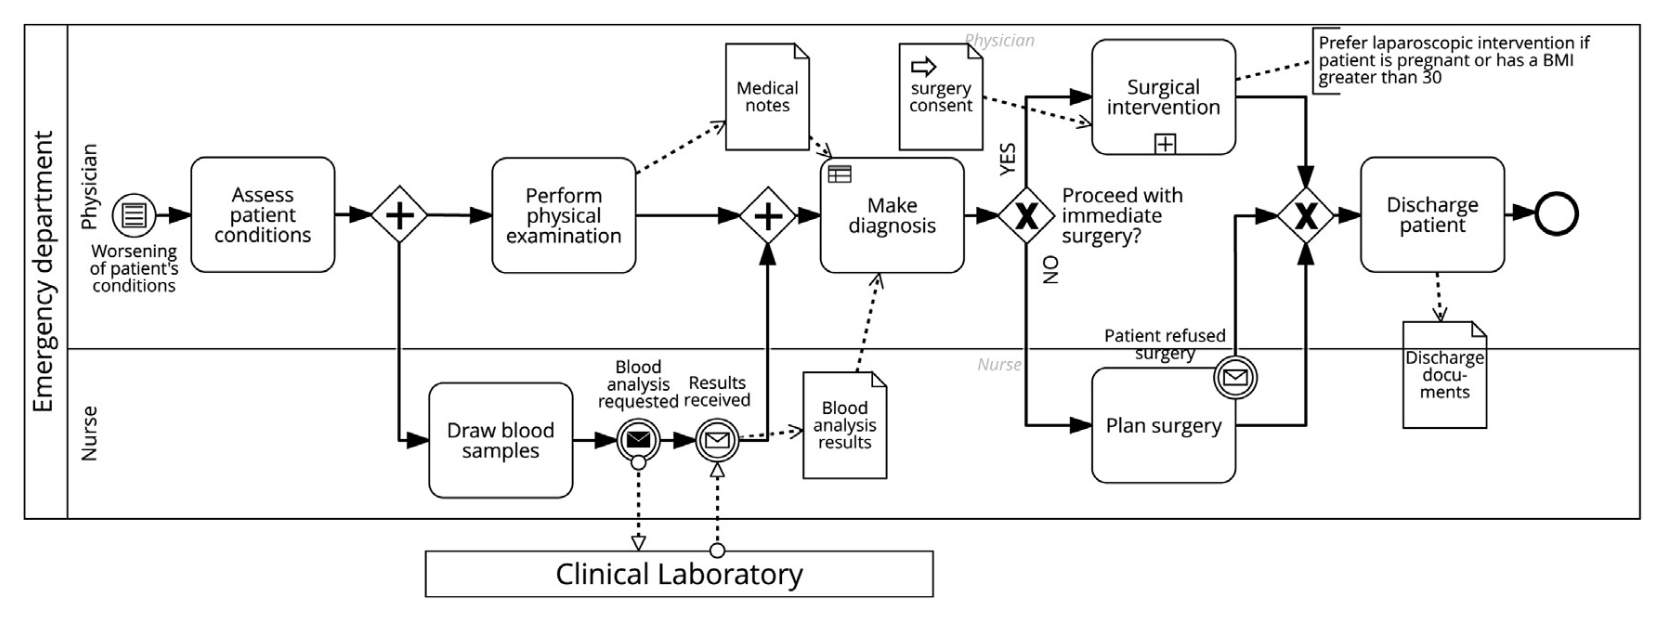
\includegraphics[width=\textwidth]{img/bpmn.png}
    \caption{Proceso simplificado de atención de urgencias en forma de diagrama de procesos BPMN. Fuente : \citetitle{pufahl_bpmn_2022}}
    \label{fig:bpmn}
\end{figure}

La Fig. 1 muestra una versión simplificada de un proceso de atención de urgencias, que se desencadena por un empeoramiento de las condiciones del paciente. Como primera tarea, el médico evalúa las condiciones del paciente.

A continuación, mientras realiza la exploración física, una enfermera extrae sangre al paciente. Las muestras de sangre se envían al laboratorio clínico para su análisis y, una vez listos, los resultados se envían de vuelta al servicio de urgencias. Con las notas de la exploración y los resultados del análisis de sangre, el médico tiene que hacer un diagnóstico. En función de los resultados, el médico realiza inmediatamente una intervención quirúrgica o la enfermera la planifica para los días siguientes, teniendo en cuenta que el paciente también puede negarse a someterse a una intervención quirúrgica. En todos los casos, el paciente es dado de alta y se le entregan los documentos de alta. Los diagramas BPMN pueden representar el flujo de control, el flujo de datos y los aspectos organizativos de un proceso con los siguientes conceptos.

\begin{itemize}
    \item Los diagramas de proceso BPMN pueden representar el flujo de control de un proceso con actividades (por ejemplo, Realizar examen físico), eventos relevantes (por ejemplo, Recibir resultados) y flujos de secuencia que los conectan. Las puertas de enlace, representadas como rombos, se utilizan para controlar los flujos de secuencia y definir comportamientos paralelos y alternativos.
    \item Las actividades pueden ser atómicas (tareas) o compuestas (subprocesos). Las tareas (por ejemplo, Realizar un examen físico) representan unidades atómicas de trabajo, mientras que los subprocesos representan actividades compuestas, que pueden colapsarse para ocultar detalles (por ejemplo, Intervención quirúrgica). BPMN presenta distintos tipos de tareas con comportamientos inherentes diferentes. Por ejemplo, las tareas de reglas de negocio se utilizan para representar tareas de toma de decisiones (p. ej., tarea Realizar diagnóstico).
    \item Los eventos externos relevantes se muestran como eventos BPMN (por ejemplo, Empeoramiento de las condiciones del paciente), que capturan los desencadenantes del proceso a los que reacciona el proceso, como mensajes, señales, condiciones (por ejemplo, Empeoramiento de las condiciones del paciente, excepciones (por ejemplo, Paciente rechazó la cirugía) y salidas producidas por el proceso (por ejemplo, Análisis de sangre solicitado).
    \item Los datos y documentos relevantes utilizados o producidos por las actividades del proceso pueden representarse con la ayuda de objetos de datos (por ejemplo, Notas médicas) o almacenes de datos cuando los datos considerados son persistentes. Se pueden adjuntar anotaciones de texto a los elementos del flujo de control para mejorar su descripción, como la anotación ''Prefer laparoscopic [...]'' asociada al subproceso Intervención quirúrgica.
    \item Las interacciones entre organizaciones pueden mostrarse mediante el concepto de pools (cada uno de ellos propietario de un proceso) (por ejemplo, el servicio de Urgencias y el laboratorio clínico) y un flujo de mensajes entre ellos.
    \item Los carriles de las agrupaciones (por ejemplo, la Enfermera y el Médico) pueden utilizarse para representar diferentes roles o sistemas que ejecutan las actividades incluidas.
\end{itemize}

\section{Análisis de la causa raíz. Cinco porqués}

Para cada efecto hay una causa.
Pero la cadena de resultados entre ambas es bastante larga y se va afinando a medida que se pasa de los insumos a las actividades, los productos, los resultados y el impacto.
En la gestión basada en resultados, el grado de control del que se disfruta disminuye a medida que se asciende en la cadena y, en consecuencia, aumenta el reto de supervisar y evaluar.

A su debido tiempo, cuando aparece un problema, es fuerte la tentación de culpar a otros o a acontecimientos externos.
Sin embargo, la raíz de los problemas suele estar más cerca de casa.

Cuando se trata de resolver un problema, es útil empezar por el resultado final, reflexionar sobre la causa y cuestionar la respuesta cinco veces.
Este enfoque elemental y a menudo eficaz de la resolución de problemas fomenta el pensamiento profundo a través del cuestionamiento y puede adaptarse rápidamente y aplicarse a la mayoría de los problemas.
Lo más obvio y directo es que la técnica de los cinco porqués está relacionada con el principio de la resolución sistemática de problemas: sin la intención del principio, la técnica sólo puede ser una cáscara del proceso.
Por lo tanto, hay tres elementos clave para el uso eficaz de la técnica de los cinco porqués:

\begin{itemize}
    \item Enunciados precisos y completos de los problemas
    \item Total honestidad al responder a las preguntas
    \item La determinación de llegar al fondo de los problemas y resolverlos
\end{itemize}

La técnica fue desarrollada por Sakichi Toyoda para Toyota Industries Corporation.

\subsection{Proceso}

El ejercicio de los cinco porqués mejora enormemente cuando lo aplica un equipo y hay cinco pasos básicos para llevarlo a cabo:

\begin{itemize}
    \item Reunir a un equipo y desarrollar el planteamiento del problema de común acuerdo. Una vez hecho esto, se decide si se necesitan más personas para resolver el problema.
    \item Se pregunta el primer "por qué" al equipo: ¿por qué se produce tal o cual problema? Probablemente habrá tres o cuatro respuestas sensatas: se anotan todas en un folio o pizarra, o con fichas pegadas a la pared.
    \item Se preguntan otros cuatro "por qué" sucesivos, repitiendo el proceso para cada afirmación en el folio, la pizarra o las fichas. Coloque cada respuesta cerca de su "padre". Se realiza un seguimiento de todas las respuestas plausibles. Cuando la pregunta "¿por qué?" no aporte más información útil, se habrá identificado la causa principal. (Si es necesario, se siguen haciendo preguntas más allá de las cinco capas arbitrarias para llegar a la causa raíz).
    \item Entre la docena de respuestas a la última pregunta "¿por qué?", se buscan las causas sistémicas del problema. Se discuten con el fin de decidir la causa sistémica más probable. Después de la sesión en equipo, es recomendable un \textit{debriefing} y mostrar el producto a los demás para confirmar que ven la lógica en el análisis.
    \item Tras determinar la causa raíz más probable del problema y obtener confirmación de la lógica que subyace al análisis, se desarrollan las medidas correctivas adecuadas para eliminar la causa raíz del sistema. Las acciones pueden (según el caso) ser emprendidas por otros, pero la planificación y ejecución se beneficiarán de las aportaciones del equipo.
\end{itemize}

\begin{figure}
    \centering
    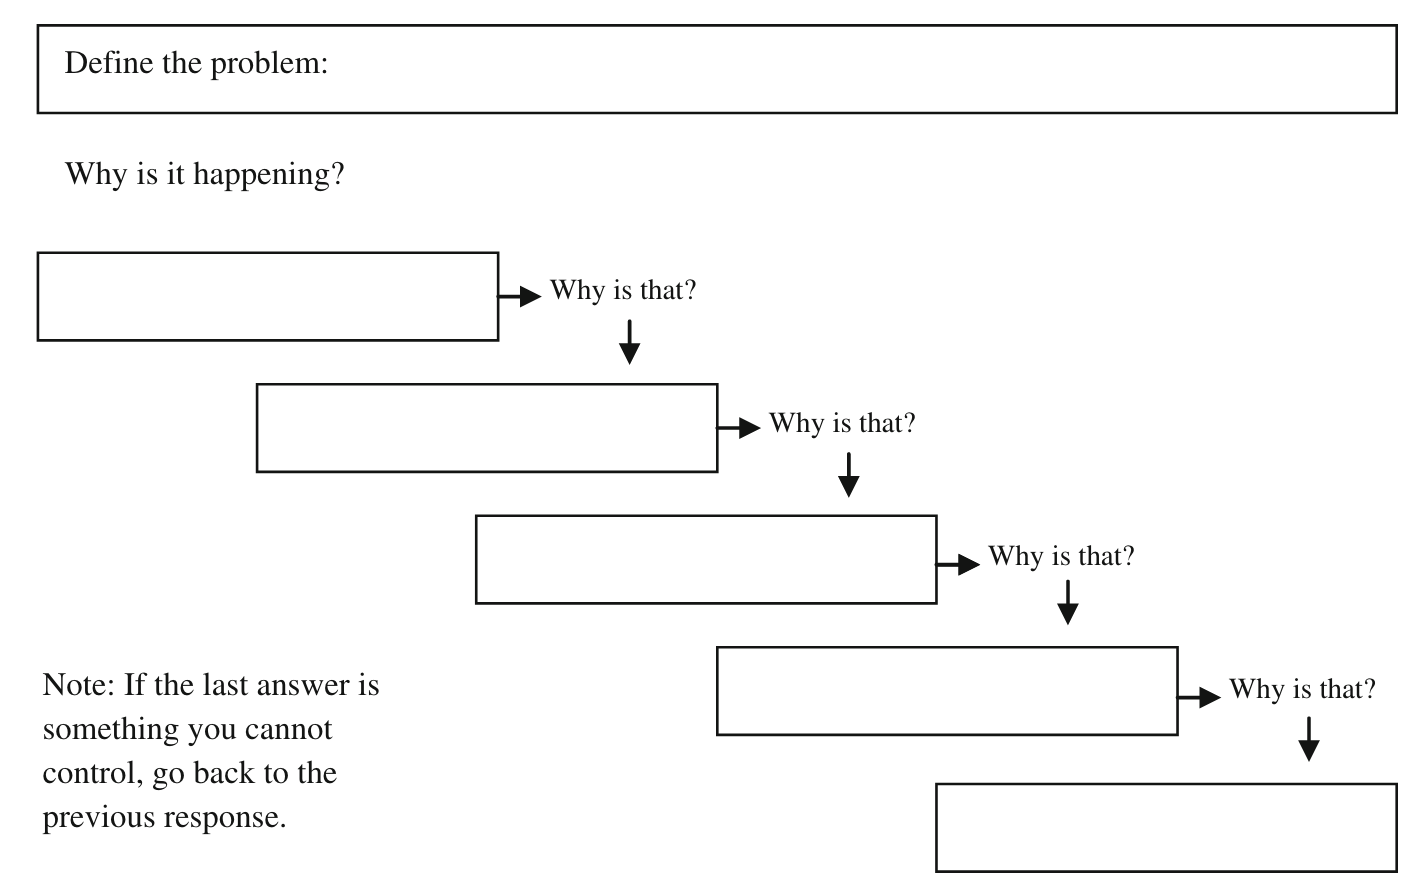
\includegraphics[width=\textwidth]{img/five-whys.png}
    \caption{Plantilla de ejemplo de los cinco porqués}
    \label{fig:five-whys}
\end{figure}

\subsection{Precauciones}

La técnica de los cinco porqués ha sido criticada por ser una herramienta demasiado básica para analizar las causas raíz con la profundidad necesaria para garantizar que las causas se solucionan.
Entre las razones de esta crítica se incluyen:

\begin{itemize}
    \item La tendencia de los investigadores a detenerse en los síntomas y no proceder a las causas profundas de nivel inferior.
    \item La incapacidad de los investigadores para ir más allá de la información y los conocimientos actuales.
    \item Falta de facilitación y apoyo para ayudar a los investigadores a formular las preguntas adecuadas.
    \item La baja tasa de repetición de los resultados: se sabe que diferentes equipos que utilizan la técnica de los cinco porqués llegan a diferentes causas para el mismo problema.
\end{itemize}

Es evidente que la técnica de los cinco porqués se resentirá si se aplica únicamente por deducción.
El proceso articulado anteriormente fomenta la verificación sobre el terreno de las respuestas a la pregunta "por qué" actual antes de pasar a la siguiente, y debería ayudar a evitar estos problemas.